\documentclass[a4paper,twoside,master.tex]{subfiles}
\begin{document}
\lecture{34}{Wednesday, April 15, 2020}{The Debye Model}

We now need to calculate the energy from the Debye model:
\begin{equation}
    U_{\text{Debye}} = 3 \frac{1}{8} \int_0^{n_D} \dd{n} 4 \pi n^2 \frac{\hbar \omega(n)}{e^{\beta \hbar \omega(n)} - 1}
\end{equation}
The prefactor of $ 3 $ counts the number of polarizations (two transverse and one longitudinal), the $ 1/8 $ is because we are only integrating over an octant, and we have left out the ground state energy from the equation for $ U $ above.
\begin{equation}
    U_{\text{Debye}} = \frac{3 \pi}{2} \int_0^{n_D} \dd{n} n^2 \frac{\hbar v \frac{\pi}{L} n}{e^{\beta \hbar v \pi n / L} - 1}
\end{equation}
Let's define $ x \equiv \frac{\beta \hbar v \pi n}{L} $ and $ \dd{x} = \frac{\beta \hbar v \pi}{L} \dd{n} $:
\begin{equation}
    U_{\text{Debye}} = \frac{3 \pi}{2} \int_0^{\frac{\beta \hbar v \pi n_D}{L}} \dd{x} x^2 \left( \frac{L}{\beta \hbar v \pi} \right)^3 \frac{1}{\beta} \frac{x}{e^x - 1}
\end{equation}
We will next define a critical ``Debye temperature'' $ \Theta_D \equiv \frac{\hbar v \pi n_D}{L k_B} = \frac{\hbar v}{k_B} \left( \frac{6 \pi^2 N}{L^3} \right)^{1/3} $:
\begin{equation}
U_{\text{Debye}} = \frac{3 \pi}{2} \frac{L^3 (k_B T)^4}{(\hbar v \pi)^3} \int_0^{\Theta_D / T} \dd{x} \frac{x^3}{e^x - 1}
\end{equation}

If the upper boundary was infinite, the solution would be easy, but it isn't. Instead, let's look in two limits. First, look at large $ T $. This seems inconsistent, since the approximations we made were meant to work for small $ T $, but it turns out there are some subtle cancellations of errors. In this limit, $ \frac{\Theta_D}{T} \to 0 $, so we can Taylor expand the integrand about $ x $:
\begin{equation}
    \frac{x^3}{e^x - 1} = \frac{x^3}{1 + x + \frac{x^2}{2} + \cdots - 1} \sim x^2 + \order{x^3}
\end{equation}
In that limit,
\begin{equation}
    U_{\text{Debye}} (T \to \infty) \approx \frac{3 \pi}{2} \frac{L^3 (k_B T)^4}{(\hbar v \pi)^3} \int_0^{\Theta / T} \dd{x} x^2 = 3 N k_B T
\end{equation}
Now remember the dispersion relation is certainly not linear for large $ k $ (large $ T $). However, for large temperature, the energy of a harmonic oscillator will go to $ \frac{1}{2} k_B T $ regardless. This is the boring limit, since we expect it to work out.


Now let's look at the (asymptotic) limit as $ T \to 0 $:
\begin{equation}
    U_{\text{Debye}}(T \to 0) \approx \frac{3 \pi}{2} \frac{L^3(k_B T)^4}{(\hbar v \pi)^3} \vdot \frac{\pi^4}{15}
\end{equation}
so
\begin{equation}
    \frac{U_{\text{Debye}}}{V} = u = \left( \frac{3 \pi^2}{30 \hbar^3 v^3}\right) (k_B T)^4
\end{equation}
This is similar to the blackbody case, although we have $ 3/30 $ rather than $ 2/30 $ due to the polarizations. Additionally, we use the phonon speed $ v $ rather than the speed of light.
\begin{equation}
    c_V \sim T^3
\end{equation}
for small $ T $.


\section{Ideal Quantum Gasses}
\label{sec:ideal_quantum_gasses}

Let's suppose we have a quantum state of $ N $ particles $ \psi(\va{r}_1, \va{r}_2 ,\cdots, \va{r}_N) $. For fermiions/bosons we need to completely antisymmetrize/symmetrize this wave function. Note that fermions/bosons are particles with half-integer/integer spin. Why is this so? This is called the Spin-Statistics Theorem. The proof involves a deeper dive into quantum field theory and is not at all obvious.

\begin{equation}
    \psi_{\{F,B\}} = X_{\{F,B\}} \sum_P \{\sigma(P), 1\} \psi(\va{r}_{P(1)}, \va{r}_{P(2)}, \cdots, \va{r}_{P(N)})
\end{equation}
where $ P $ are the permutations of $ \{1, \cdots, N\} $ and $ \sigma $ is $ +1 $ for an even permutation and $ -1 $ for an odd permutation and $ X $ is some normalization factor. If the original wave function can be written as
\begin{equation}
    \psi(\va{r}_1, \cdots, \va{r}_N) = \prod_{i=1}^{N} \psi_{\alpha_i}(\va{r}_i)
\end{equation}
(a product of single-particle quantum states), then
\begin{equation}
    \psi_{\{F,B\}} = X_{\{F,B\}} \sum_P \{\sigma(P), 1\} \prod_{i=1}^{N} \psi_{\alpha_i}(\va{r}_{P(i)})
\end{equation}
In the Fermion case, this is called the ``Slater determinant''.

Suppose the Hamiltonian is of the form
\begin{equation}
    H_N = \sum_{j=1}^{N} H_j,
\end{equation}
a sum of individual Hamiltonians for each particle, and each $ H_j $ are identical. If this is true,
\begin{equation}
    H_n \psi_{\{F,B\}} = E \psi_{\{F,B\}} = \sum_{j=1}^{N} \epsilon_{\alpha_j} \psi_{\{F,B\}}
\end{equation}
so
\begin{equation}
    Z = \sum_{\{\alpha\}}' e^{- \beta \sum_{j=1}^{N} \epsilon_{\alpha_j}} = \sum_{\{\alpha\}}' \prod_{j=1}^{N} e^{- \beta \epsilon_{\alpha_j}}
\end{equation}
The sums which have a prime by them are special. These are sums over all quantum states subject to the (anti)symmetrization constraint. This is hard, because it doesn't allow us to look at an individual particle without considering all the others to maintain symmetry. However, there is a better way of dealing with this, but it requires a clever change of notation:

\begin{figure}[h]
    \centering
    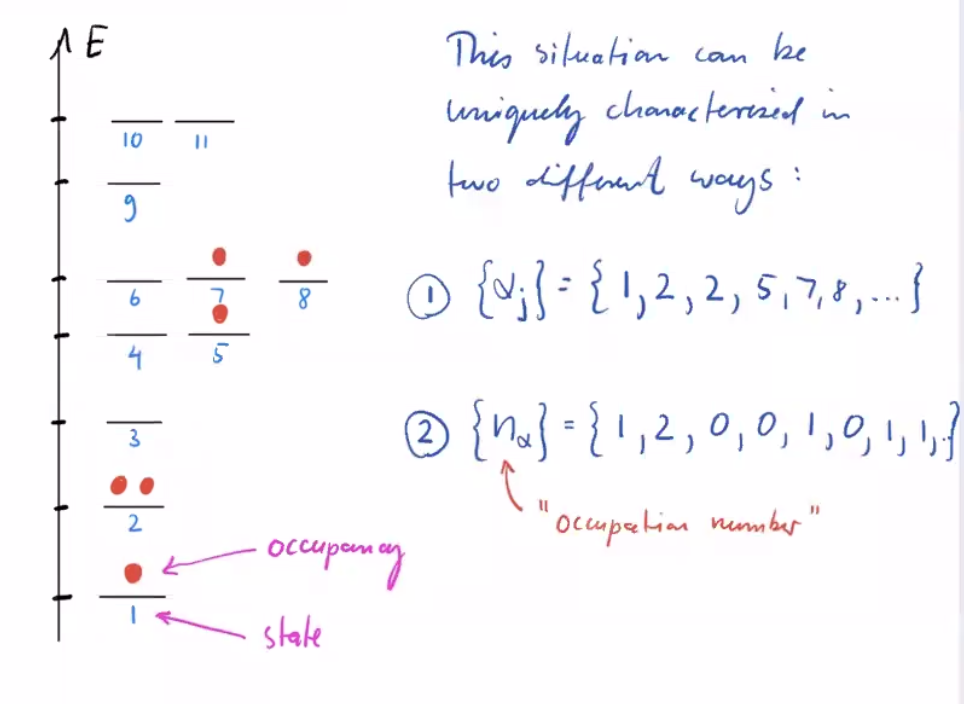
\includegraphics{figures/lec_34_occupancy.png}
    \caption{Using Occupancy Number to lable states}
    \label{fig:lec_34_occupancy}
\end{figure}

\end{document}
